\documentclass{article}
\usepackage{amsmath}
\usepackage[spanish, es-tabla]{babel}
\usepackage{caption}
\DeclareCaptionLabelFormat{cont}{#1~#2\alph{ContinuedFloat}}
\captionsetup[ContinuedFloat]{labelformat=cont}
\usepackage{graphicx}
\usepackage[style=authoryear,backend=biber]{biblatex}
\addbibresource{referencia.bib}

\begin{document}
		\begin{center}
		{\bfseries Universidad Sim\'on Bol\'ivar\par}
		{\bfseries Mec\'anica Cl\'asica II (FS4212)\par}
		\vspace{0.5cm}
		{\scshape\Huge Calculo de un oscilador de tipo Van der Pol \par} %  MODIFICAR EL NOMBRE
		\vspace{0.5cm}
		{\scshape\large Profesor: Ra\'ul Isea \par}
		{\scshape\large Estudiante: Arquimedes Chauran \qquad Carnet: 1910061 \par}
	\end{center}
	
	\section{Ecuaci\'on de Van der Pol}
	
	Es una ecuacion que surge de analizar ciertos circuitos electrónicos. Aplicada para estudiar las oscilaciones en sistemas mecánicos y eléctricos, como en también en la determinación de ritmos cardíacos \autocite{goldstein2014},\autocite{ku}.
	
	\begin{equation*}
		m\frac{d^2x}{dt^2}-e(1-x^2)\frac{dx}{dt}+m\omega_0^2x=0
	\end{equation*}
	
	Tambi\'en se encuentra con un t\'ermino oscilatorio \autocite{goldstein2014}.
	
	\begin{equation*}
		m\frac{d^2x}{dt^2}-e(1-x^2)\frac{dx}{dt}+m\omega_0^2x=F\cos\omega_Dt
	\end{equation*}
	
	En el desarrollo de los cálculos se escogi\'o trabajar con la primera de estas ecuaciones.
	
	\section{Lagrangiano para la ecuaci\'on de Van der Pol}
	
	Como es una ecuaci\'on de segundo orden lineal en la velocidad, podemos en principio hacer usar una funci\'on de disipaci\'on para tomar en cuenta el t\'ermino no lineal. Entonces, se puede escribir la ecuacion de Lagrange como sigue \autocite{greiner2010}
	
	\begin{equation*}
		\frac{d}{dt}\left(\frac{\partial \mathcal{L}}{\partial \dot{q}}\right)-\frac{\partial \mathcal{L}}{\partial q}=\frac{\partial D}{\partial \dot{q}}
	\end{equation*}
	
	Donde, para el caso la ecuaci\'on del oscilador de Van der Pol, obtenemos que
	
	\begin{equation*}
		\mathcal{L}=\frac{1}{2}m\dot{x}^2-\frac{1}{2}m\omega_0^2x^2 \qquad y \qquad
		D=e(1-x^2)\dot{x}^2
	\end{equation*}
	
	Se plante\'o encontrar una funci\'on hamiltoniana que describiera la din\'amica del oscilador de Van der Pol. Sin embargo, debido a la particularidad de ser una ecuaci\'on diferencial no lineal. En concreto, contiene un producto cruzado de la posición al cuadrado con la velocidad. Por tanto, no se encontr\'o una forma de incluirlo en la obtención de las ecuaciones can\'onicas. En las referencias consultadas, unicamente se consideraban t\'erminos disipativos con coeficientes constantes en la velocidad y se encontraba el hamiltoniano vía la ecuacion de Hamilton-Jacobi \autocite{ola2013}.
	
	\section{\'Orbita}
	
	La \'orbita de un sistema particular es su trayectoria en el espacio de las fases.
	
	Para la \'orbita en el espacio de las fases de la ecuaci\'on de Van der Pol, existe una variacion apreciable en su forma que depende del parámetro e. 
	
	\begin{figure}[h!]
		\centering
		\ContinuedFloat*
		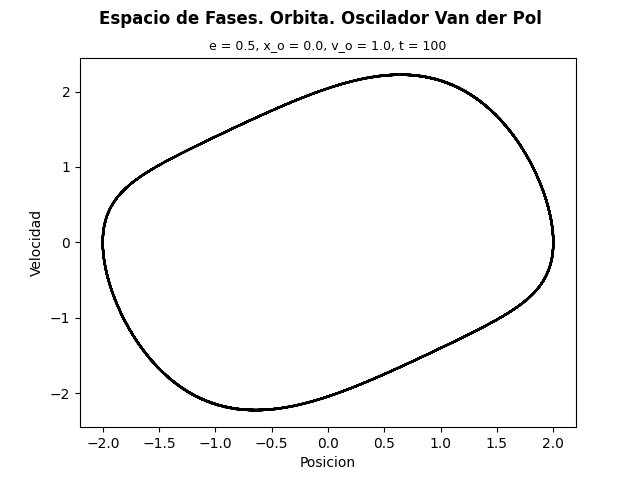
\includegraphics[width=0.7\linewidth]{ESPACIO FASE. ORBITA. e=0.5}
		\caption{Gr\'afico de la orbita del oscilador de Van der Pol para los par\'ametros e=0.5, $x_0=0.0$ y $v_0=1.0$.}
	\end{figure}
	
	\begin{figure}[h!]
		\centering
		\ContinuedFloat
		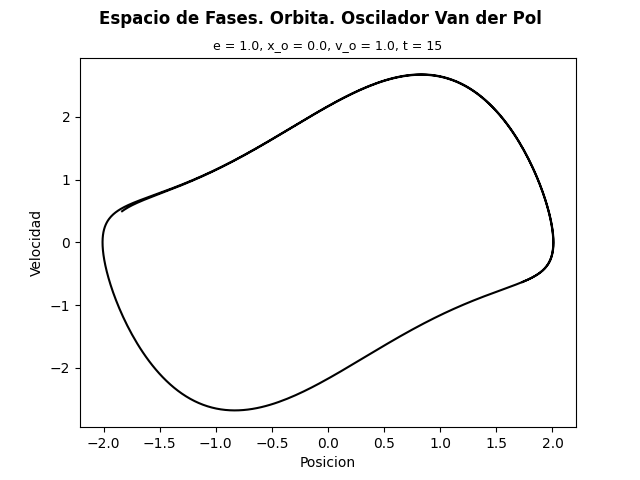
\includegraphics[width=0.7\linewidth]{ESPACIO FASE. ORBITA. e=1.0}
		\caption{Gr\'afico de la orbita del oscilador de Van der Pol para los par\'ametros e=1.0, $x_0=0.0$ y $v_0=1.0$.}
	\end{figure}
	
	\begin{figure}[h!]
		\centering
		\ContinuedFloat
		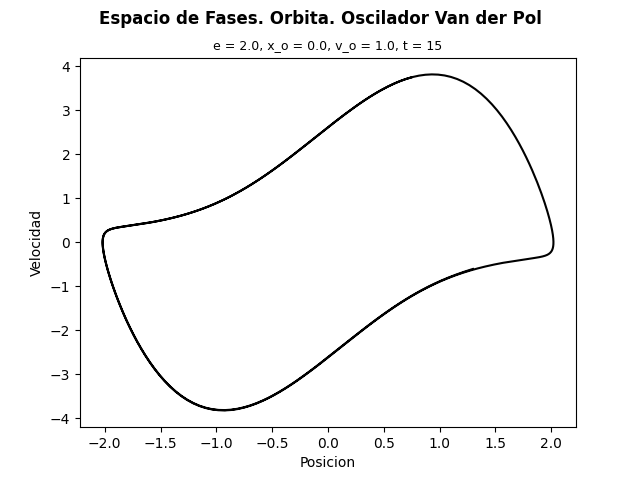
\includegraphics[width=0.7\linewidth]{ESPACIO FASE. ORBITA. e=2.0}
		\caption{Gr\'afico de la orbita del oscilador de Van der Pol para los par\'ametros e=2.0, $x_0=0.0$ y $v_0=1.0$.}
	\end{figure}
	
	El aumento del parámetro e achata o modifica la orbita. Por otro lado, se observa que mientras mas pequeño se vuelve el parámetro e, la orbita tiende a la curva que describe un oscilador armónico. Un resultado coherente con la forma de la ecuacion de Van der Pol.
	
	\newpage
	
	
	\section{Diagrama de Poincare}
	
	Para los diagramas de Poincare se tomaron puntos del espacio fase cada 10 segundos en un primer caso y en un segundo caso se tomaron puntos cada 20 segundos. Estos est\'an marcados por un punto rojo en las figuras siguientes. Podemos notar una cierta tendencia propia del car\'acter oscilatorio de la ecuaci\'on; es decir, vemos como los puntos se agrupan en sitios particulares de la orbita.\newline
	
	Es de notar como la distribuci\'on de puntos de los diagramas de Poincare se juntan en zonas particulares para el tiempo en el que se toman. En principio, podríamos determinar por tanteo el periodo de oscilación acercando estos puntos. En otros palabras, se busca un valor del tiempo para el cual se toman los puntos de tal manera que estos se acerquen lo suficiente.\newline
	
	Es apreciable como los puntos en la figura 3a se distancian. Lo cual, claramente indica que tomar intervalos de 20s no produce una aproximación buena del periodo del oscilador.
	
	\begin{figure}[h!]
		\centering
		\ContinuedFloat*
		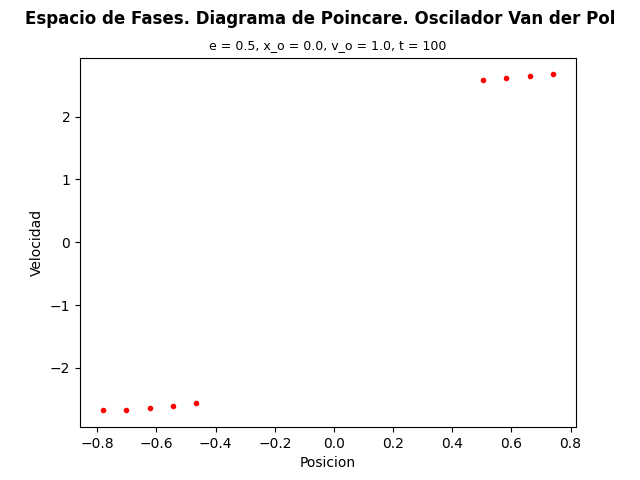
\includegraphics[width=0.8\linewidth]{DIAGRAMA DE POINCARE 1}
		\caption{Gr\'afico del diagrama de Poincare para puntos cada 10s de la oscilaci\'on del oscilador de Van der Pol para los par\'ametros e=1.0, $x_0=0.0$ y $v_0=1.0$. Se marcan en rojos los puntos.}
	\end{figure}
	
	\begin{figure}[h!]
		\centering
		\ContinuedFloat
		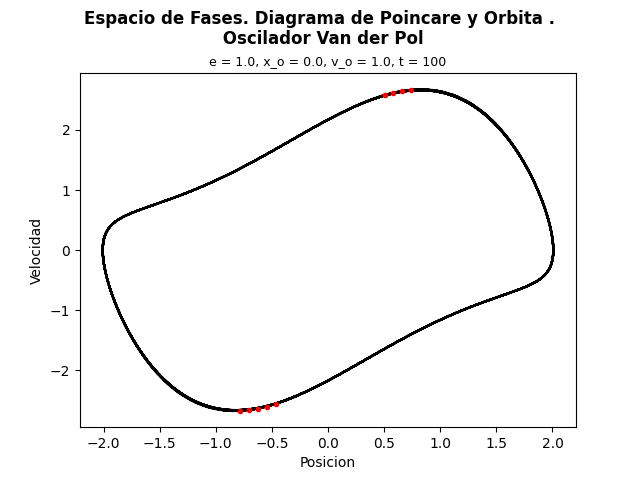
\includegraphics[width=0.8\linewidth]{DIAGRAMA DE POINCARE Y ORBITA 1}
		\caption{Gr\'afico del diagrama de Poincare con la orbita respectiva para puntos cada 10s de la oscilaci\'on del oscilador de Van der Pol para los par\'ametros e=1.0, $x_0=0.0$ y $v_0=1.0$. Se marcan en rojo los puntos.}
	\end{figure}
	
	\begin{figure}[h!]
		\centering
		\ContinuedFloat*
		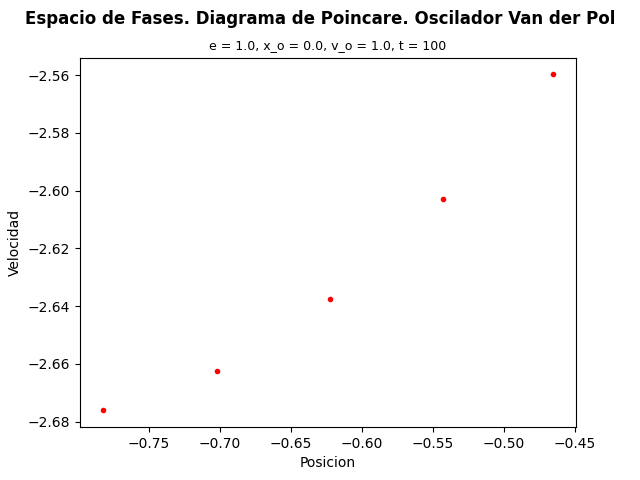
\includegraphics[width=0.8\linewidth]{DIAGRAMA DE POINCARE 2}
		\caption{Gr\'afico del diagrama de Poincare para puntos cada 20s de la oscilaci\'on del oscilador de Van der Pol para los par\'ametros e=1.0, $x_0=0.0$ y $v_0=1.0$. Se marcan en rojo los puntos.}
	\end{figure}
	
	\begin{figure}[h!]
		\centering
		\ContinuedFloat
		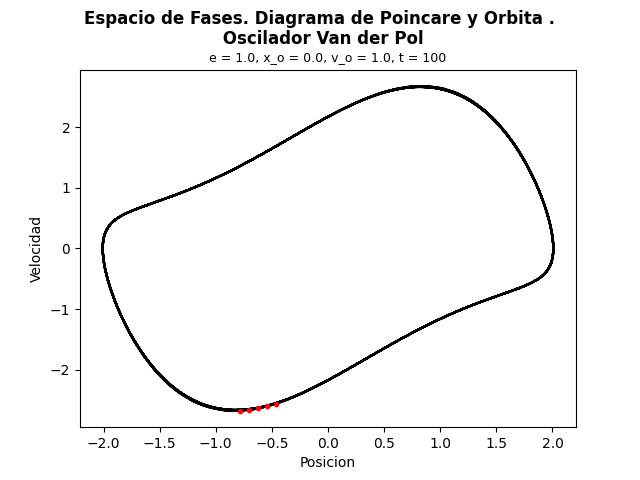
\includegraphics[width=0.8\linewidth]{DIAGRAMA DE POINCARE Y ORBITA 2}
		\caption{Gr\'afico del diagrama de Poincare con la orbita respectiva para puntos cada 20s de la oscilaci\'on del oscilador de Van der Pol para los par\'ametros e=1.0, $x_0=0.0$ y $v_0=1.0$. Se marcan en rojo los puntos.}
	\end{figure}
	
	\newpage
	
	\section{Gráfica de velocidad cero}
	
	Considerare como gr\'afica de velocidad cero a la gr\'afica con condiciones iniciales $x_0\neq0,\quad v_0=0$. En este sentido, tenemos tanto la representación en el espacio de fases como v vs. t.\\
	
	En este caso, lo mas apreciable es que aunque el sistema comienza en con velocidad cero, se recupera el carácter oscilatorio de los soluciones ya vista anteriormente. También cabe destacar que se comienza fuera del equilibrio. Si se iniciara en el equilibrio ($x_0=0,\quad v_0=0$) no ocurre ningún movimiento puesto que las condiciones iniciales se comportan como un punto de equilibrio estable.\\
	
	La figura 4a muestra en principio como a pesar de las condiciones iniciales particulares elegidas, el sistema descrito por la ecuaci\'on de Van der Pol tiende a la forma que se muestra. Este tipo de comportamientos podrian ser útil estudiarlos si se requiere que un sistema particular tienda siempre a un modo de funcionamiento indistintamente de donde inicie. \\
	
	\newpage
	
	\begin{figure}[h!]
		\centering
		\ContinuedFloat*
		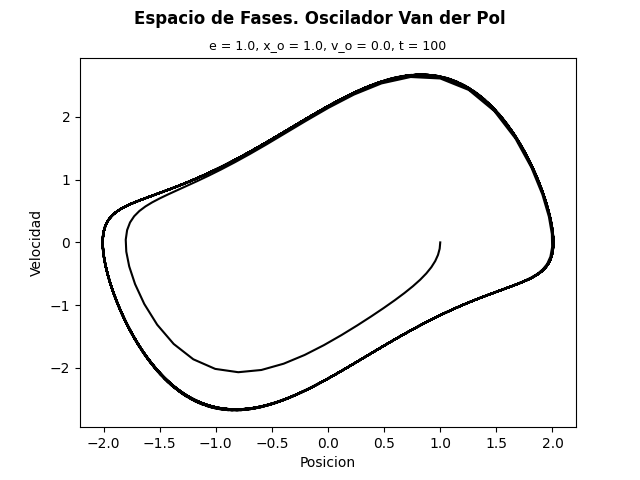
\includegraphics[width=0.8\linewidth]{VELOCIDAD CERO 1}
		\caption{Gr\'afico de velocidad cero en el espacio de las fases del oscilador de Van der Pol para los par\'ametros e=1.0, $x_0=1.0$ y $v_0=0.0$.}
	\end{figure}
	
	\begin{figure}[h!]
		\centering
		\ContinuedFloat
		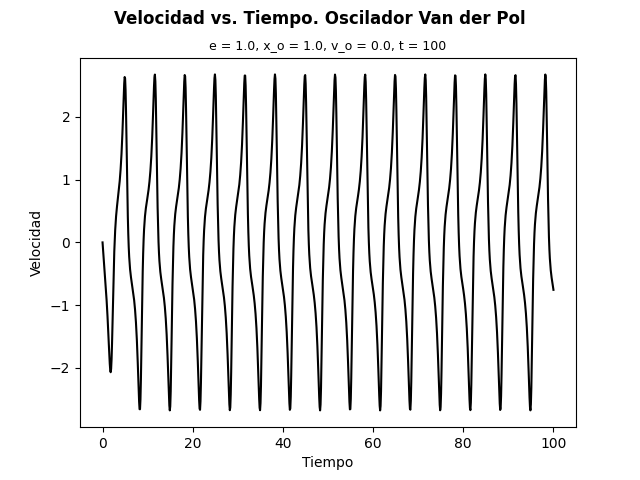
\includegraphics[width=0.8\linewidth]{VELOCIDAD CERO 2}
		\caption{Gr\'afico de velocidad cero en velocidad vs. tiempo de las fases del oscilador de Van der Pol para los par\'ametros e=1.0, $x_0=1.0$ y $v_0=0.0$.}
	\end{figure}
	
	\newpage
	
	\printbibliography
	
\end{document}